\documentclass[12pt]{article}
\usepackage[utf8]{inputenc}
\usepackage{graphicx}
\usepackage{hyperref}
\usepackage{listings}
\usepackage{xcolor}
\usepackage{float}
\usepackage{geometry}

\geometry{
    a4paper,
    margin=2.5cm
}

\definecolor{codegreen}{rgb}{0,0.6,0}
\definecolor{codegray}{rgb}{0.5,0.5,0.5}
\definecolor{codepurple}{rgb}{0.58,0,0.82}
\definecolor{backcolour}{rgb}{0.95,0.95,0.92}

\lstdefinestyle{mystyle}{
    backgroundcolor=\color{backcolour},   
    commentstyle=\color{codegreen},
    keywordstyle=\color{magenta},
    numberstyle=\tiny\color{codegray},
    stringstyle=\color{codepurple},
    basicstyle=\ttfamily\footnotesize,
    breakatwhitespace=false,         
    breaklines=true,                 
    captionpos=b,                    
    keepspaces=true,                 
    numbers=left,                    
    numbersep=5pt,                  
    showspaces=false,                
    showstringspaces=false,
    showtabs=false,                  
    tabsize=2
}

\lstset{style=mystyle}

\title{Project Stacy: AI Healthcare Assistant}
\author{Pranav Verma}
\date{\today}

\begin{document}

\maketitle
\tableofcontents
\newpage

\section{My Journey}

\subsection{Why I Did This}
I started this project after talking with a diverse group of individuals—students, working adults, and even my neighbors, who were all having a hard time accessing mental health services. I had one simple goal in mind: to create a digital companion that is always available, non-judgmental, and actually empathetic.

\section{From Idea to Reality}

\subsection{Early Development Days}
In the early stages, I spent my days prototyping, planning, and having many discussions. I experimented with various AI models and discussed different approaches to the user interface, with one thing in mind: I wanted to make my app feel like a friendly and caring companion, not just a tool.

I decided to go with Qwen 2.5, because I did not have enough powerful hardware to run the big and heavy models. Not only was it smart, but it could also detect emotional signals.

\begin{figure}[H]
  \centering
  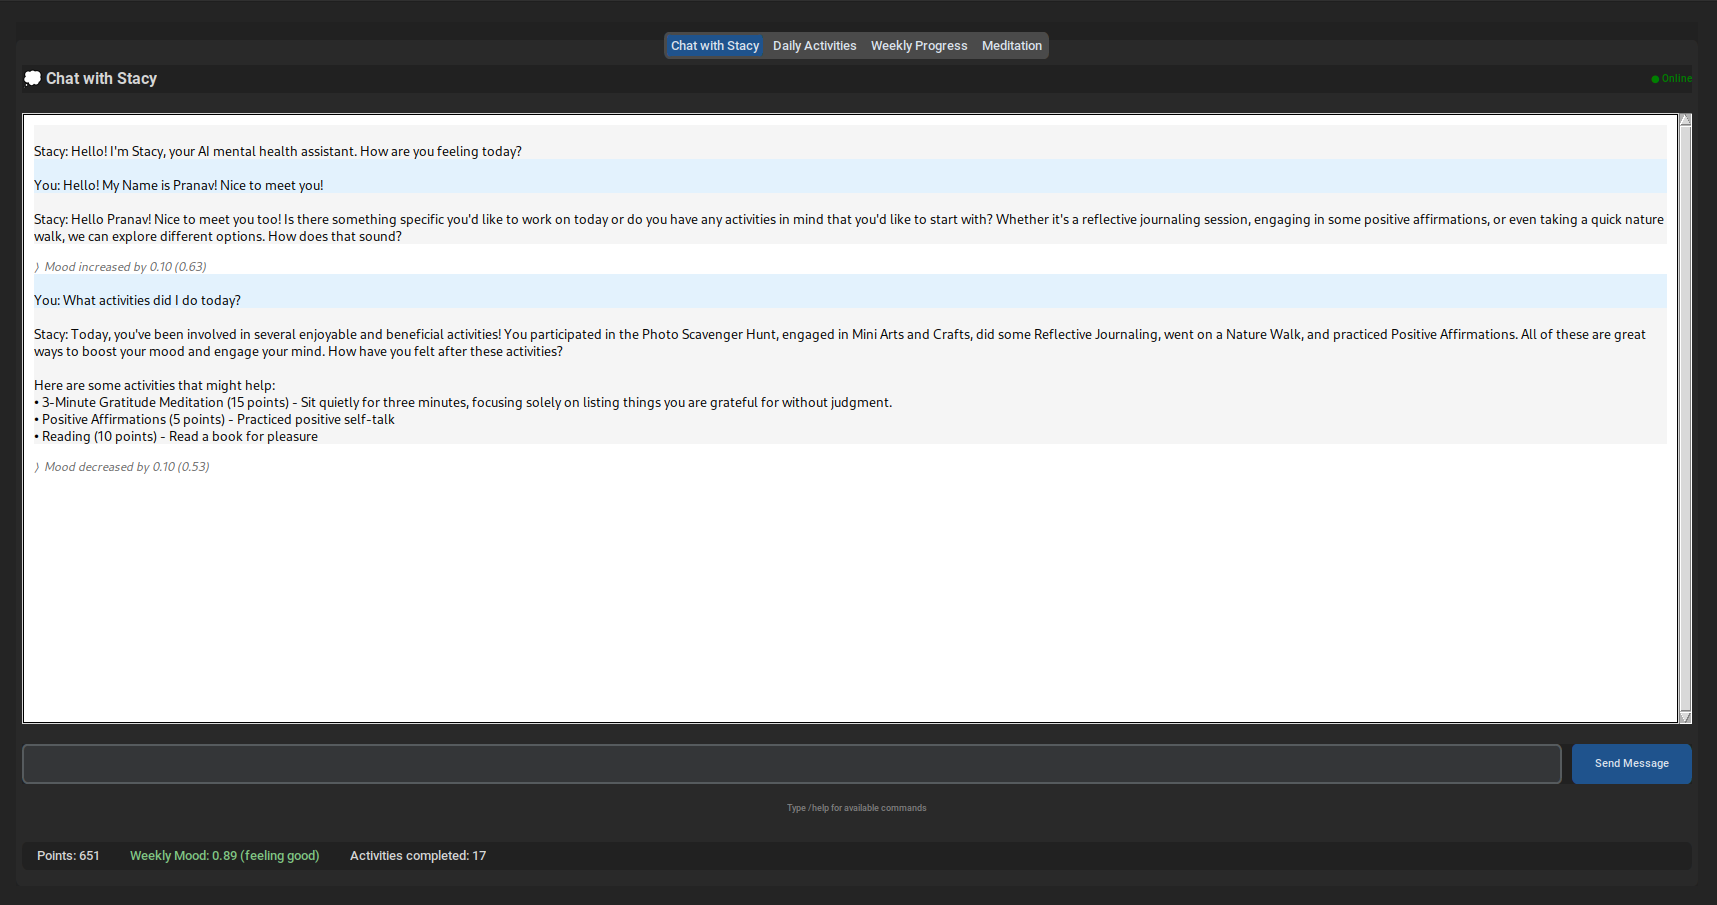
\includegraphics[width=1\textwidth]{../images/Chat.png}
  \caption{Chat interface with Stacy, showing the AI assistant's empathetic responses}
\end{figure}

\section{Core Features: The Pillars of My Application}

\subsection{The AI Buddy}
Stacy is more than a program; after months of fine-tuning, she has become a sympathetic presence that intuitively adapts to your mood. If you are anxious about an upcoming presentation or just need a calming presence, Stacy picks up on your mood and responds accordingly—offering reassurance or listening when you need to talk.

\subsection{Mood Monitoring and Analysis}
Rather than having users manually rate their mood, I developed a system that detects emotional patterns through normal conversations. Over time, Stacy learns about your behavior patterns and, when she detects stress, gently reminds you or suggests something helpful—providing subtle support like a thoughtful friend.

\begin{figure}[H]
  \centering
  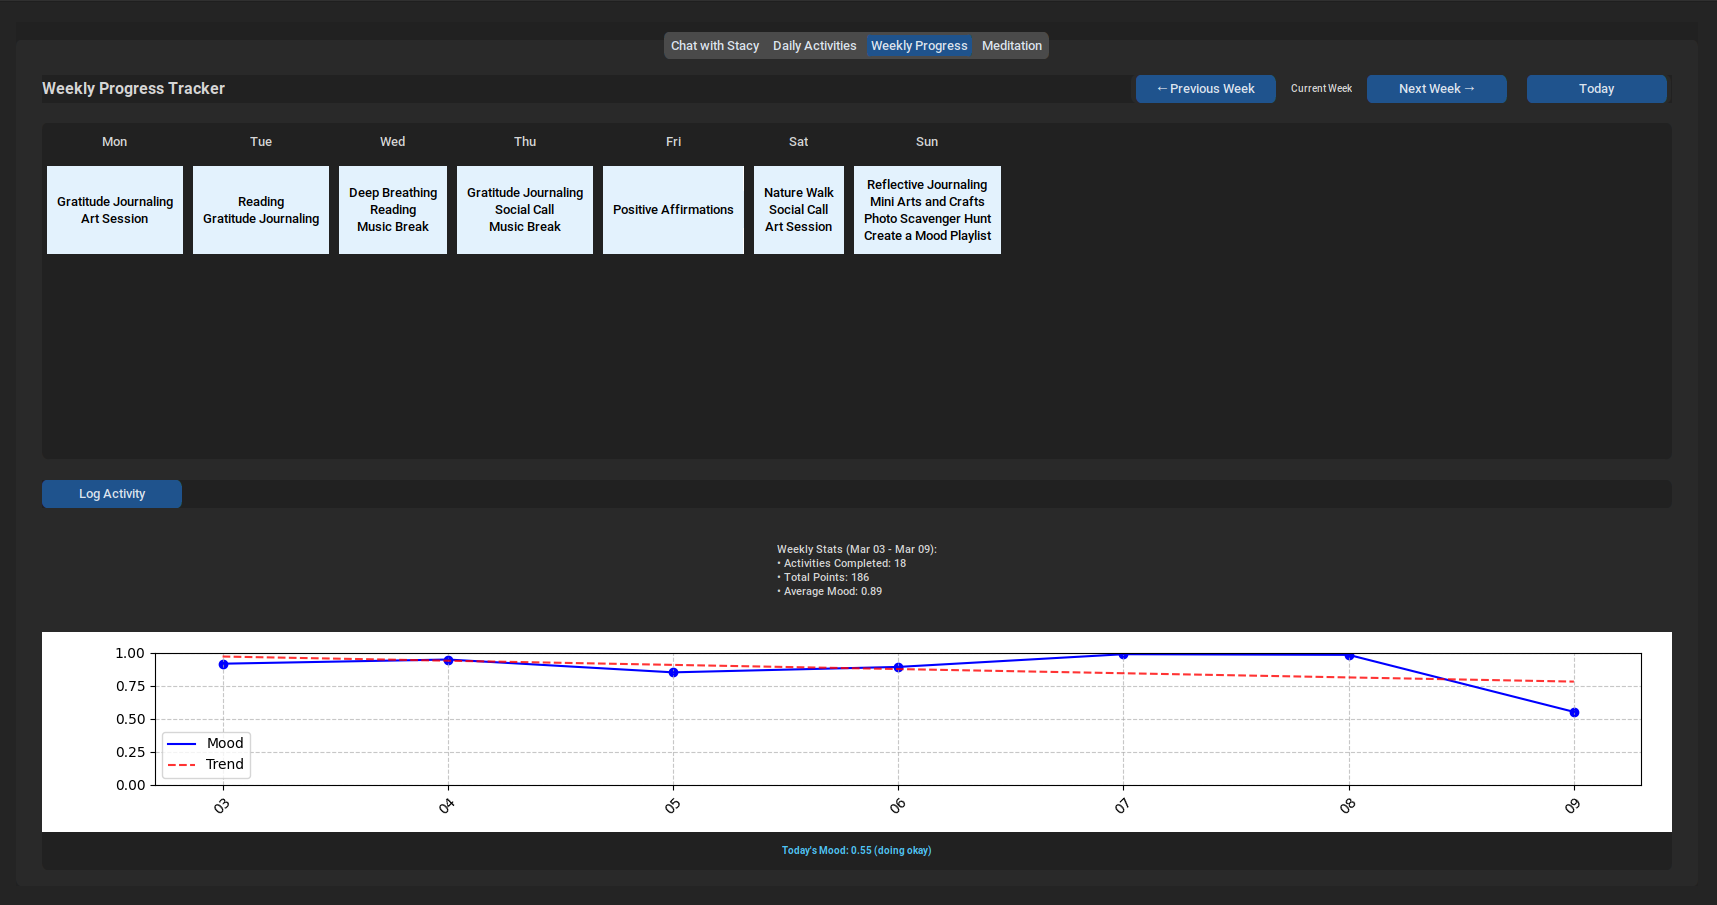
\includegraphics[width=0.8\textwidth]{../images/Progress-Tracker.png}
  \caption{Weekly progress tracker showing mood analysis and activity completion}
\end{figure}

\subsection{The Activity System}
My activity system is based on the belief that small accomplishments can have a significant impact on mood. The system suggests activities that are tailored to your current mood and energy levels, ranging from quick breathing exercises to creative challenges. Not only do you earn points by completing these activities, but you also feel supported and validated.

\begin{figure}[H]
  \centering
  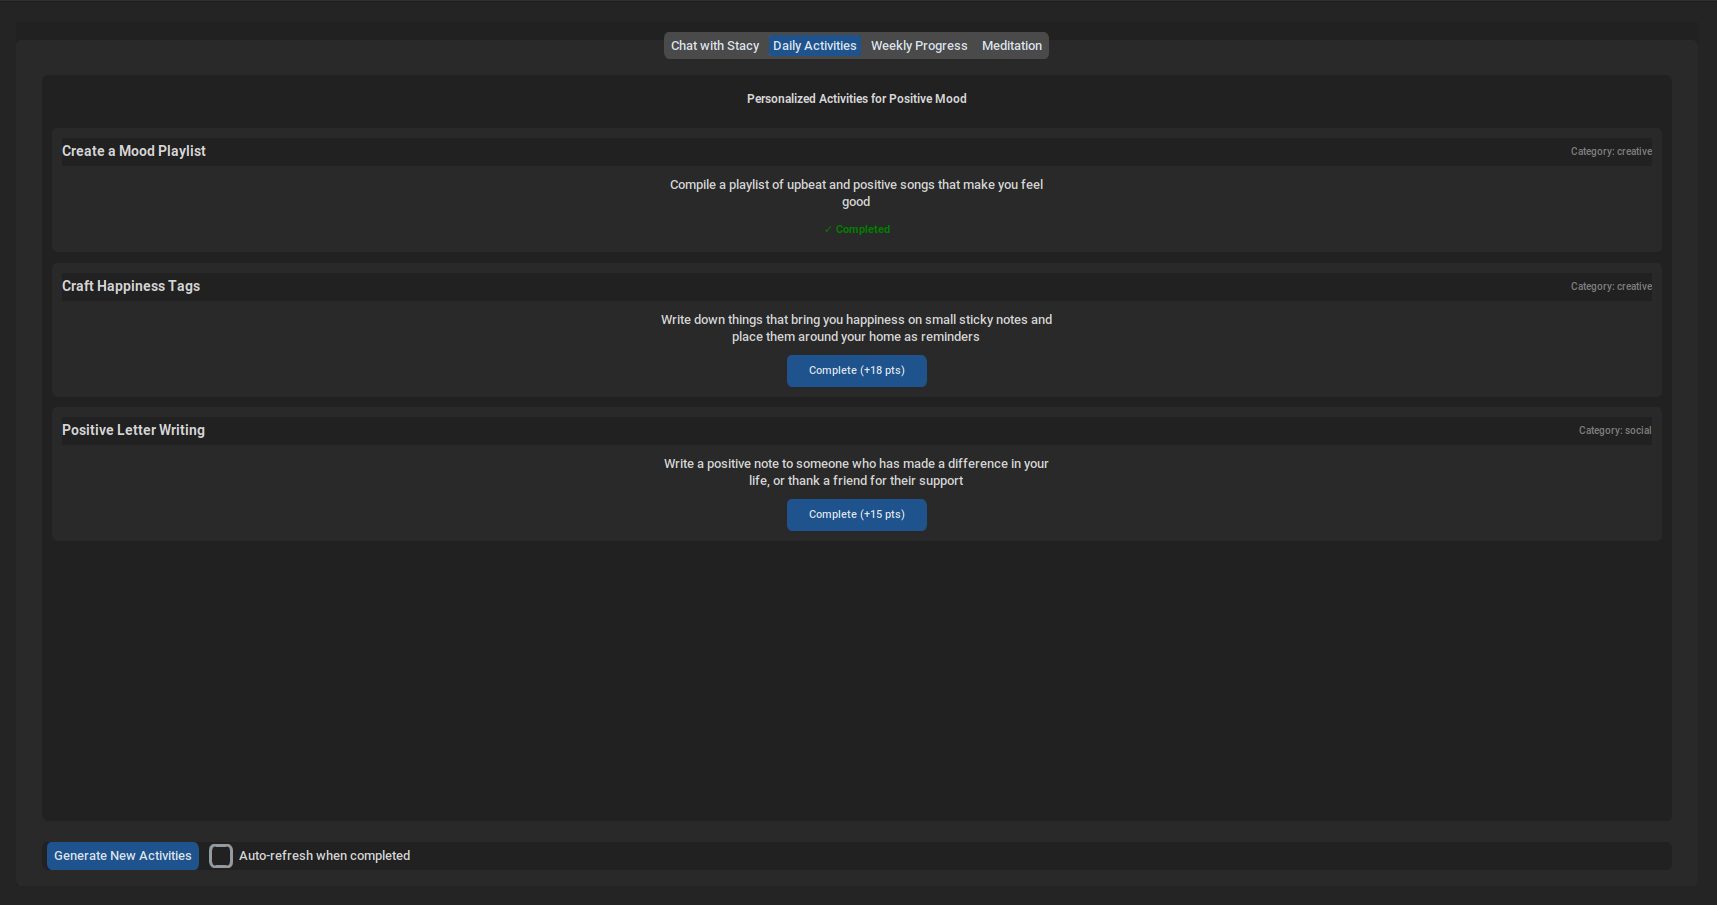
\includegraphics[width=0.8\textwidth]{../images/Activities.png}
  \caption{Activity recommendations tailored to the user's current mood and needs}
\end{figure}

\section{Technical Insights: In the Background}

\subsection{Building the Brain}
The artificial intelligence engine that powers Stacy is a sophisticated system. When users interact with her, the app seamlessly translates messages, maintains conversational context, recognizes emotional subtleties, detects psychological concerns, and generates responses—all within milliseconds.

\subsection{Data Privacy and Protection}
Privacy has been a priority since day one. Everything that users input—conversations, mood insights, and activity history—is securely stored on the device. I employed encrypted SQLite storage and strict cryptographic methods to make sure your data is as private as a personal diary.

\section{Overcoming Development Hurdles}

\subsection{The AI Response Challenge}
Initially, Stacy struggled to interpret emotional cues effectively. A simple remark about feeling overwhelmed would sometimes prompt a generic response. To fix this, I developed an empathy module that evaluates emotional tone, considers past interactions, assesses urgency, and ensures responses are contextually appropriate. This significantly improved the natural feel of conversations.

\subsection{The Performance Puzzle}
Early versions experienced noticeable delays in mood analysis. I resolved this by adding predictive pre-fetching, caching frequent interactions, offloading computationally expensive tasks to background threads, and integrating smooth loading animations. These optimizations resulted in near-instant responses.

\subsection{The Privacy Dilemma}
My early models stored conversation history in plain text—a major security issue that I quickly addressed. I transitioned to a local-first design with end-to-end encryption, secure memory management, on-demand data deletion, and privacy-conscious analytics, ensuring complete user confidentiality.

\subsection{The Context Memory Problem}
Previously, Stacy would forget important details from ongoing conversations, leading to fragmented interactions. I addressed this by implementing a memory hierarchy: short-term memory for active sessions, medium-term memory for recent conversations, and long-term recall for recurring patterns. A conversation anchoring mechanism also strengthens Stacy's ability to maintain coherence.

\subsection{The Engagement Challenge}
Initially, user engagement with activity suggestions was low. I enhanced the system by introducing adaptive difficulty levels, rewarding micro-progress, tailoring recommendations based on real-time conversation cues, and allowing flexible scheduling. These improvements made activities more engaging and accessible.

\begin{figure}[H]
  \centering
  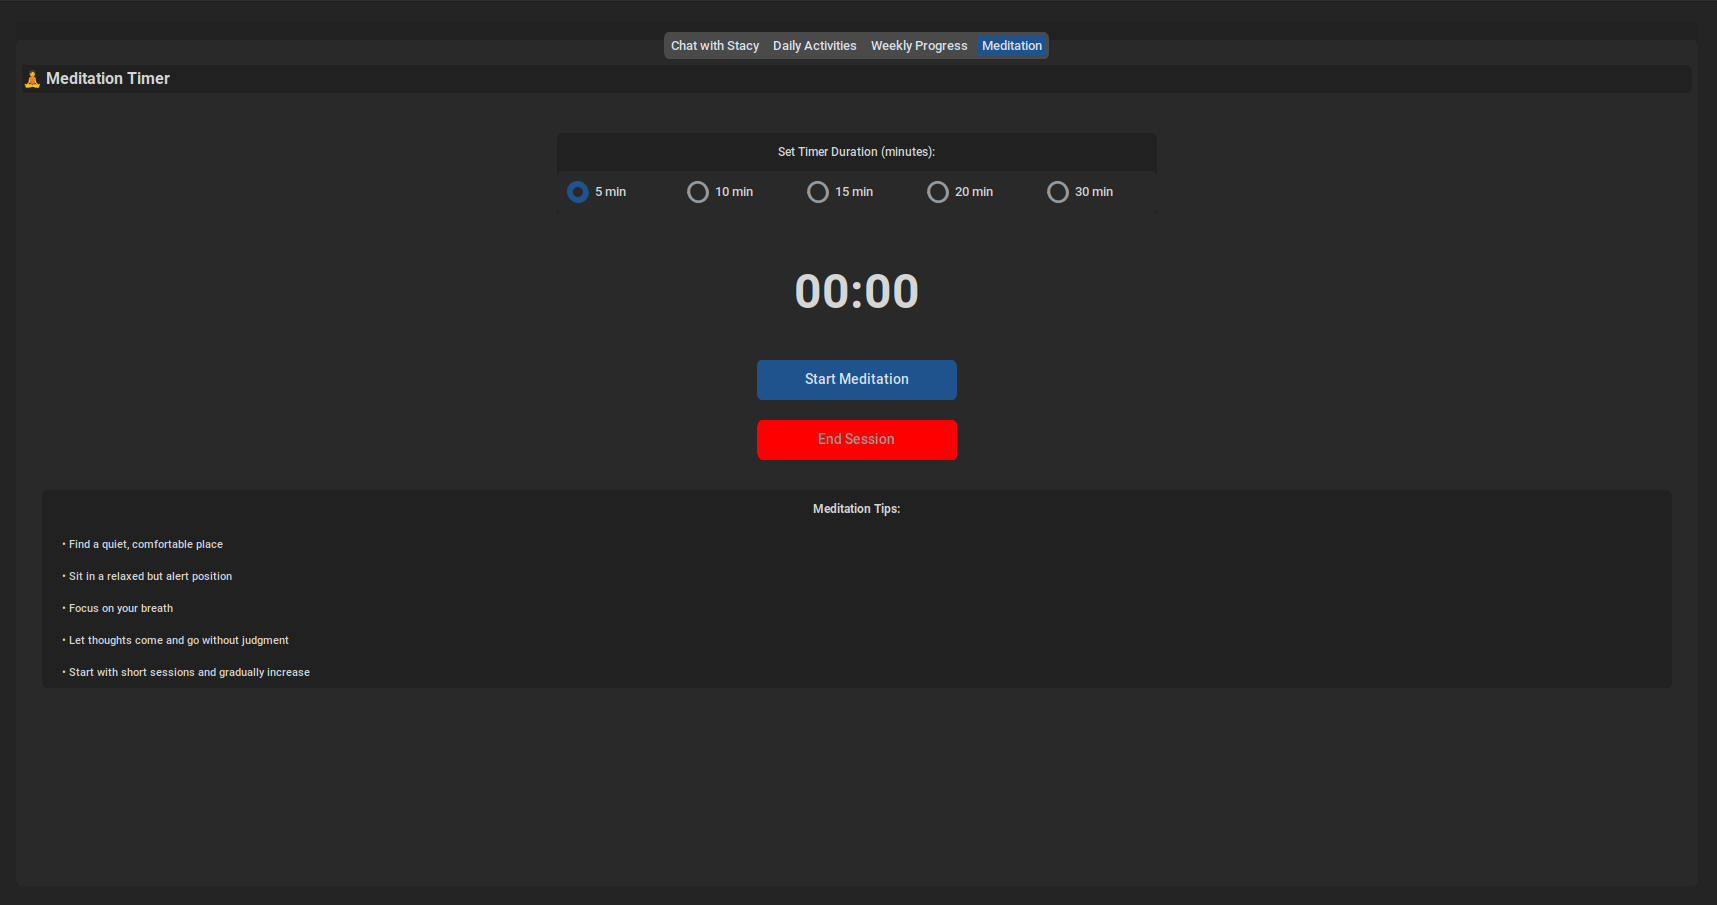
\includegraphics[width=0.8\textwidth]{../images/Meditation.png}
  \caption{Meditation timer feature to help users practice mindfulness}
\end{figure}

\subsection{Lessons Learned}
This journey reinforced the importance of balancing technical excellence with a genuine user experience. Frequent testing with diverse user groups, prioritizing privacy from the outset, and ensuring meaningful, human-like interactions were all crucial in shaping Stacy.

\section{Real-World Impact}

\subsection{User Stories}
After the project reached it's final stage, I decided to try it out in the wild. I gave a copy of Stacy to anyone and everyone that I felt needed it. That includes my dad, who is constantly in stress from work, my mom, who again is under stress from house work, and other users aswell. All of them reported that they feel better after using Stacy.

\subsection{Continuous Improvement}
Learning is an ongoing process. User feedback has guided improvements such as more personalized activity suggestions, enhanced crisis response handling, improved memory retention, and even more natural conversations.

\subsection{Open Source Contribution}
I've made Stacy available as an open-source project on GitHub at \url{https://github.com/PranavVerma-droid/AI-Healthcare}. By making the code accessible to everyone, I hope to encourage collaboration, innovation, and wider adoption of mental health technology. Anyone can contribute to Stacy's development, adapt it for specific needs, or use it as a foundation for similar initiatives.

\section{Technical Implementation Details}

In this section, I highlight some of the key technical components that power Stacy. Below are short excerpts from the code used in the project.

\subsection{AI Response Generation}
The core logic for generating Stacy's conversational responses is implemented in the \texttt{AIHelper} class. For example:

\begin{lstlisting}[language=Python, caption=AI Response Handler, label=lst:ai_helper]
# file: ai_helper.py

def get_response(self, user_input):
    # Build detailed context including today's activities and recent chats
    todays_activities = self.activity_manager.get_todays_activities()
    # ...existing code...
    
    daily_context = "Today's Activities: " + todays_activities
    # ...existing code...
    
    messages.append({"role": "system", "content": system_prompt})
    messages.append({"role": "user", "content": user_input})
    
    response = self.client.chat(model=self.model, messages=messages)
\end{lstlisting}

\subsection{Sentiment Analysis}
Stacy's empathetic responses are driven by real-time sentiment analysis. The \texttt{SentimentAnalyzer} class uses an AI service with a fallback mechanism:

\begin{lstlisting}[language=Python, caption=Sentiment Analysis, label=lst:sentiment]
# file: sentiment.py

def analyze_sentiment(self, text: str) -> Tuple[float, str, float]:
    messages are [
        {"role": "system", "content": "Analyze the sentiment of the following text."},
        # ...existing code...
    ]
    
    response = self.client.chat(model=self.model, messages=messages)
\end{lstlisting}

\subsection{Local Data Management and Privacy}
Stacy maintains user data locally with SQLite. The \texttt{Database} class initializes the required tables while enforcing local security:

\begin{lstlisting}[language=Python, caption=Database Handler, label=lst:database]
# file: database.py

def _init_db(self):
    conn = sqlite3.connect(self.db_path)
    cursor = conn.cursor()
    
    # Create tables for chat_history, mood_tracking, activities, user_progress, and activity_notes
    cursor.execute("CREATE TABLE IF NOT EXISTS chat_history (...);")
    # ...existing code...
\end{lstlisting}

\subsection{UI Interaction and Asynchronous Processing}
The responsive UI built with CustomTkinter utilizes threading to process AI input without freezing the interface:

\begin{lstlisting}[language=Python, caption=Main Interface, label=lst:main]
# file: main.py

def send_message(self):
    user_input = self.message_input.get().strip()
    
    # Handle commands or dispatch AI response asynchronously
    threading.Thread(target=self.process_message, args=(user_input,)).start()
\end{lstlisting}

\end{document}
